\section{Rendu temps réel}

Notre objectif est d'avoir un rendu en temps réel, c'est à dire une fréquence d'image au minimum de 30 par secondes. Si tout le bâtiment devrait être calculé à chaque image il est clair que nous aurions pas un rendu assez rapide. Comme expliqué dans le chapitre \emph{Analyse} de ce rapport, la librairie WebGL que l'on utilise (three.js) offre du \textit{Backface et Frustum culling}. Grâce à ces avantages il est déjà plus simple d'effectuer un rendu temps réel.

Une solution imaginée pour gagner en performance était d'effectuer une découpe du bâtiment en de nombreux morceaux (Schéma en figure \ref{fig:rendering-slice}). Chacune de ces pièces serait sauvegardée dans deux versions différentes: une en haute qualité et l'autre en moins bonne qualité. A partir de là l'idée était de mettre en place un système \emph{LoD (Level of Detail)} \cite{wiki-lod}. Ce qui signifie qu'on charge le modèle en bonne qualité seulement si la caméra est proche de ce dernier, sinon on charge le modèle en qualité plus basse. Cependant les tests effectuées n'ont pas montrés un réel gain de performance. Il a été conclu que ceci était du au \textit{culling} géré par la three.js.

\begin{figure}
\centering
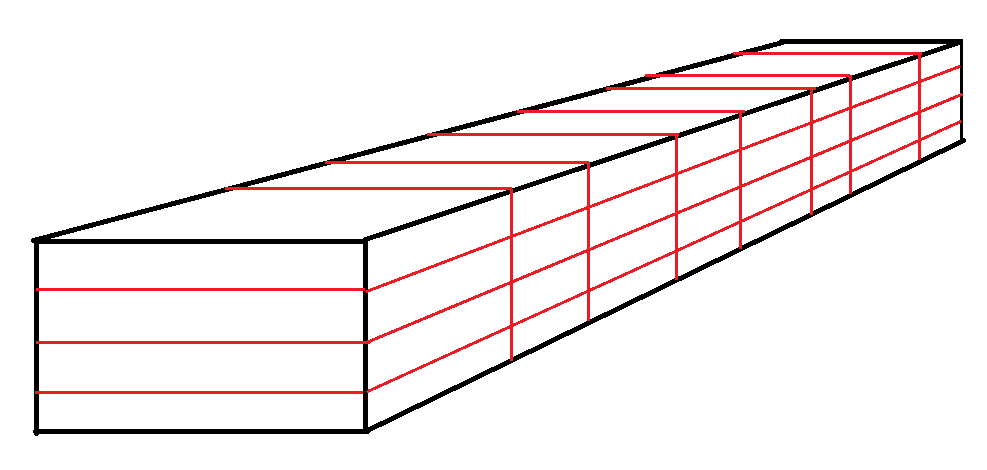
\includegraphics[width=0.7\linewidth]{rendering-Slice}
\caption{Schéma d'une découpe du bâtiment possible.}
\label{fig:rendering-slice}
\end{figure}

\subsection{Textures indexées}
Un problème de performance s'est montré après avoir exporté la version texturée du modèle. Afin d'appliquer plusieurs textures sur un même objet avec \textit{Autodesk 3ds max} il faut utiliser des \emph{Multi/Sub-Object Material}. C'est en fait une liste de matériaux indexés, on l'applique à notre objet et ensuite on définit quel indice du matériau la face affiche. Cependant après avoir utilisé ce genre de matériau sur le modèle, le nombre d'image par seconde sur mobile est descendu aux alentours de deux ou trois. L'analyse a fait remarquer que le \textit{renderer} est appelé environs 5000 fois et sans les textures il est appelé 30 à 40 fois. Le problème vient en fait que pour chaque fragment il doit changer de texture et c'est cette partie qui lui prend énormément de temps. La solution adopté est de classer notre géométrie par textures, comme cela le \textit{renderer} ne doit changer qu'un nombre limité de fois de textures et le nombre d'image par seconde est de nouveau en dessus de 30.

\subsection{Matériel utilisé}
L'application offre au minimum 30 images par seconde. Mais le nombre d'images par seconde n'est pas très objectif sans les informations du matériel utilisé. Les tests effectués sur un ordinateur portable se sont fait avec un \emph{HP EliteBook 8570w}:

\begin{description}[align=right, labelwidth=3cm]
	\item [OS] Microsoft Windows 10
	\item [Chipset]	Mobile Intel® QM77 Express Chipset
	\item [CPU] 3rd Generation Intel® CoreTM i7 Quad-Core
	\item [GPU] A NVIDIA Quadro K2000M
\end{description}

Pour les tests sur smartphone c'est un \emph{Motorola Nexus 6} qui a été utilisé:

\begin{description}[align=right, labelwidth=3cm]
	\item [OS] 	Android OS v6.0 (Marshmallow)
	\item [Chipset]	Qualcomm Snapdragon 805
	\item [CPU] Quad-core 2.7 GHz Krait 450
	\item [GPU] Adreno 420
\end{description}
